%%%%%%%%%%%%%%%%%%%%%%%%%%%%%%%		CHAP 2		%%%%%%%%%%%%%%%%%%%%%%%%%%%%%%%

\chapter{The ANNIE Experiment}
\label{cha:2}

 As more neutrino data become available, lack of knowledge of the fine details of the %
 neutrino-nucleus interactions begins to limit the physics reach of future experiments. 
 For instance, final-state neutron abundance from pure neutrino interactions are currently %
 poorly known and difficult to measure.
 Data on neutron yield in relation to energy and direction of final-state muons can be used to %
 better constrain nuclear models of neutrino interaction %
 physics and are an essential input to Monte Carlo models, used for calculating %
 detection efficiencies, expected background rates, accurate limits, and confidence levels.
 The count of neutrons can also be used to reject contamination by atmospheric %
 neutrino interactions in proton decay experiments and in a sample of diffuse supernova %
 background neutrinos and may also help to statistically address wrong-sign contamination %
 in oscillation analyses.
 In addition to helping understand fundamental neutrino-interaction physics, tagging events %
 by the presence and number of final-state neutrons can provide physics analyses with a better %
 handle for signal/background separation and even allow for discrimination between %
 different types of neutrino interactions.

 \begin{wrapfigure}{L}{0.5\textwidth}
   \centering
   
\includegraphics[scale=.2]{pics/logo_2}
   \caption{Logo of the ANNIE experiment.}
   \label{fig:logo}
 \end{wrapfigure}

 A study on final-state neutron abundance can be accomplished by the %
 \textbf{A}ccelerator \textbf{N}eutrino \textbf{N}eutron \textbf{I}nteraction \textbf{E}xperiment %
 (ANNIE), which will provide a complementary measurement of neutron yields in %
 neutrino-nucleon interactions.
 The ANNIE experiment is a prototype neutrino detector currently taking data at the %
 Fermi National Accelerator Laboratory (FNAL, Fermilab), in Chicago, USA.
 It consists of a small water Cherenkov detector, placed at the former location of %
 the SciBooNE experiment~ref[Phys. Rev. D 78 (2008) 112004] and %
 deployed on the intense Booster Neutrino Beam (BNB).
 An upstream forward Veto and a downstream Muon Range Detector (MRD) are also installed %
 in the hall.
 The experiment aims to be a test bed for many new technologies, as the gadolinium-doped water %
 and the use of early prototype Large Area Picosecond Photodetectors (LAPPDs).
 Neutron tagging in Gd-loaded water may play a significant role
 in reducing backgrounds from atmospheric neutrinos in next generation 
 proton-decay searches using megaton-scale Water Cherenkov detectors, like Hyper-Kamiokande~ref.
 Similar techniques might also be useful in the detection of supernova neutrinos. 
 Accurate determination of neutron tagging efficiencies will require a 
 detailed understanding of the number of neutrons produced by neutrino interactions 
 in water as a function of momentum transferred.
 This accuracy can be achieved by using precision timing, thank to the LAPPDs, to localise %
 interaction vertices in the small fiducial volume of the detector.
 The ANNIE experiment will be an innovative application of these devices demonstrating %
 their feasibility for Water Cherenkov neutrino detectors.
 
 The experiment is planned to proceed in two stages, spread over five years:
 \begin{description}
   \item[\bfseries Phase I] a partially-instrumented test-beam run using only Photomultipliers %
     (PMTs) for the purpose of measuring critical neutron backgrounds to the experiment;
   \item[\bfseries Phase II] a longer run with a more fully-instrumented detector %
     where incremental research and development for the LAPPDs and %
     accompanying fast electronics will be fulfilled, as long as the expansion of the %
     photodetector coverage (both LAPPDs and PMTs) required.
 \end{description}

 \emph{Year 1} will focus on the R\&D, particularly on the development of the Data Acquisition %
 system, along with the testing in water of the first model of LAPPD. 
 Installation of the first LAPPDs and a significant fraction of the additional PMTs, as %
 well as the calibration system, will take place in \emph{Year 2}.
 Data-taking would commence in \emph{Year 3} and continue through \emph{Year 5}, %
 with the physics reach of the detector improving as the fraction of LAPPDs increases over time.
 Publication of derived results would occur by the end of \emph{Year 5}.
 
 This thesis takes place at the beginning of \emph{Year 1}, where testing of the Phase I %
 experimental setup is tested and R\%D is undertaken.

 \section{Physics of the experiment}

 As established previously, detection of final state neutrons from nuclear interactions %
 would have a transformative impact on a wide variety of neutrino physics measurements.
 Nevertheless there are major limitations on the effective execution of neutron tagging %
 techniques, for both sides of Physics:
 \begin{itemize}
   \item theoretically, large theoretical uncertainties on the nuclear mechanisms that %
     produce neutrons in GeV-scale neutrino interactions are not still clear;
   \item experimentally, the neutron yield hasn't been satisfactorily measured yet.
 \end{itemize}

 The physics of neutrino-nucleus interactions depends on the complex interplay of multiple particles %
 and different energy scales, and it can vary greatly among target materials. 
 It is also known that the number and type of nucleons ejected from the interaction provides a %
 valuable constraint on models of neutrino-nucleus interactions. 
 ANNIE can study neutron yields from mostly-pure neutrino interactions separately %
 and will study neutron yields in relation to the energy and direction of final-state muons
 with respect to the original neutrino. 

\begin{wrapfigure}{R}{0.5\textwidth}
  \centering
\begin{fmffile}{ccqe}
  \begin{fmfgraph*}(80,50)
    \fmfleft{i2,i1}
    \fmfright{o2,o1}
    \fmf{fermion}{i1,v1,o1}
    \fmf{photon,label=$W$}{v1,v2}
    \fmf{fermion}{i2,v2,o2}
    \fmflabel{$\nu_\mu,\bar{\nu}_\mu$}{i1}
    \fmflabel{$p,n$}{i2}
    \fmflabel{$\mu^+,\mu^-$}{o1}
    \fmflabel{$n,p$}{o2}
  \end{fmfgraph*}
\end{fmffile}
\vspace{5pt}
\caption{CC interaction of a neutrino with a nucleon, producing the corresponding lepton. %
This interaction is called Quasi Elastic.}
\label{fig:ccqe}
\end{wrapfigure}

 The principal process to be considered at the first order is the charged current (CC) exchange, %
 which yields a proton (neutron) from the neutrino (anti-neutrino) interaction, %
 and neutral current (NC) interactions, which produce either protons or neutrons. 
 Higher-order processes and multi-scale nuclear physics, including secondary (p,n) scattering %
 of struck nucleons within the nucleus, charge exchange reactions of energetic hadrons %
 in the nucleus (e.g., $\pi^- \, p\rightarrow n \, \pi^0$), and Meson Exchange Currents (MEC), where %
 the neutrino interacts with a correlated pair of nucleons, all modify these expectations.
 The theory describing these interactions is under development and is often weakly constrained %
 by the available data. 
 One of the main result published by the MiniBooNE collaboration~ref, concerns the Charged Current %
 Quasi-Elastic interactions.
 The first double differential cross section for CCQE interactions are better described by models %
 including two-body currents, where low-energy neutrinos scatter off correlated pairs of %
 nucleons.
 A relevant predicted consequence of two-body currents is higher multiplicity of final-state %
 A key handle in understanding neutrino-nucleus interaction is the number and type of nucleons %
 ejected from the interaction.
 \textcolor{red}{More on this. Ask Teppei?}

 The search for a delayed signal from neutron capture on Gadolinium (Gd) salts dissolved in water %
 is a promising technique for detecting final state neutrons.

 It is therefore critical that we experimentally characterise the probability of producing zero %
 (P(N=0)), one (P(N=1)), or multiple (P(N>1)) neutrons from a neutrino interaction, as a function %
 of both interaction type and momentum transfer.
 Even moderately energetic neutrons ranging from tens to hundreds of MeV will quickly lose energy %
 by collisions with free protons and oxygen nuclei in water. 
 Once thermalised, the neutrons undergo radiative capture, combining with a nearby nucleus to %
 produce a more tightly bound final state, with excess energy released in a gamma-ray ( ) cascade. 
 Gd-doped water enhances the capture cross-section compared to pure water %
 (49,000 barns compared with 0.3 barns on a free proton) and, since the cascade happens %
 at higher energies (8 MeV vs 2.2 MeV), it produces enough optical light to be reliably detected in %
 a large target volume.

 ANNIE will require collecting data from sufficient neutrino interactions to make accurate %
 statements about neutron yield in an inclusive sample of neutrino interactions. 
 The primary goal is to measure distributions of neutron yield from muon neutrino charged %
 current interactions versus 6various kinematic observables such as momentum transfer. 
 It is expected that this would require on the order of 10K neutrino interactions considering %
 the efficiencies and acceptances of the experimental setup ($\sim$10\,\% of the interactions %
 in the detector). 
 This corresponds to one year of data. 
 With additional statistics (additional 2 years of data) and improved detector performance, %
 the more demanding goal of studying neutron yields for specific event classes can be met.

 \textcolor{red}{What can happen inside the tank? Cosmic, beam and stuff, what they triggers, %
   how they can be seen, how the detectors react.}

 \section{Neutrino beam}

 ANNIE is run on axis from the \emph{Booster Neutrino Beam} (BNB), which deploys %
 \np{8.89}~GeV protons accelerated from the Fermilab booster operating at 15~Hz.
 The primary beam from the \emph{Linac} uses protons accelerated to 8 GeV kinetic energy %
 by the Fermilab booster. 
 Selected batches containing approximately \np{5e12} protons are extracted %
 and bent toward a beryllium target via dipole magnets.
 Each spill is composed of 81 bunches of protons, approximately 6~ns wide each %
 and 19~ns apart, for a total spill duration of $\np{1.6}~\mu$s.
 As far as the detector is concerned, the neutrino beam is seen to arrive with a spill frequency of 15~Hz, %
 divided in pulse train, around 1~s apart each other.

 Beam proton trajectories and positions are monitored on a pulse-by-pulse basis.
 Upstream of the target, the primary proton beam is monitored on a pulse-by-pulse basis %
 using four systems: %
 two toroids measuring its intensity (protons-per-pulse), beam position monitors %
 (BPM) and a multi-wire chamber determining the beam width and position, %
 and a resistive wall monitor (RWM) measuring both the time and intensity of the beam spills.
 A logic signal is also generated by the last device for every intensity peak.
 It is employed to trigger the experiment in correspondence of each spill.
 The BNB is dealt in detail in the appendix~\ref{app:A}.

\begin{wrapfigure}{R}{0.5\textwidth}
%\begin{figure}[]
  \centering
  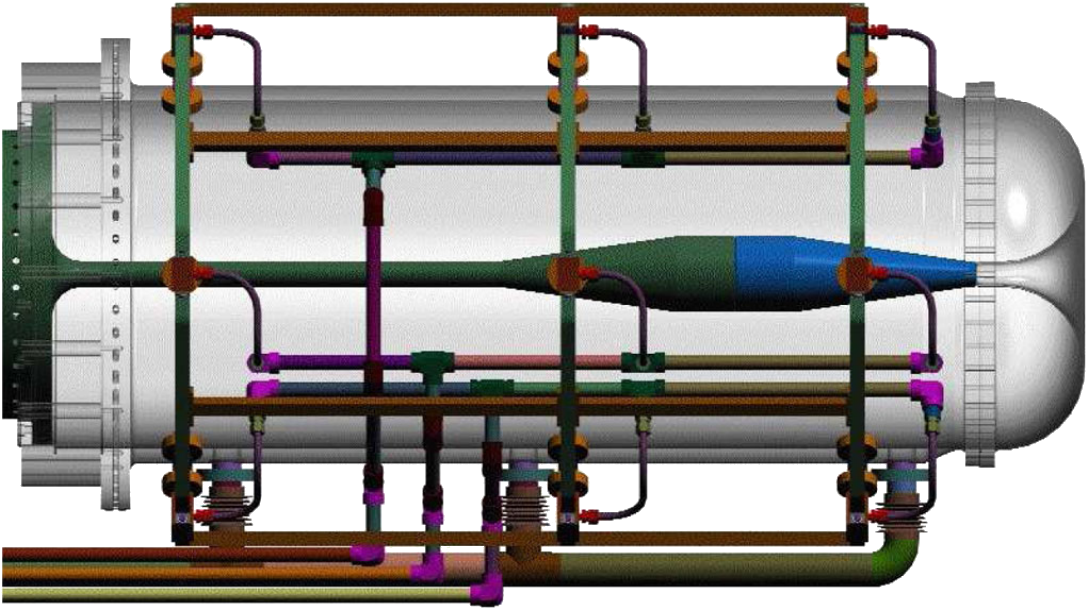
\includegraphics[scale=.2]{pics/bnbhorn}
  \caption{BNB horn system.}
  \label{fig:bnbhorn}
\end{wrapfigure}

Hadronic interactions of the protons with the target material produce a beam of %
secondary mesons, mostly pions and kaons. 
A magnetic focusing horn, shown in Fig.~\ref{fig:bnbhorn}, surrounds the beryllium target, %
bending and sign-selecting the secondary particles emitted along the direction pointing to the hall.
The focusing is produced by the toroidal magnetic field present in the air volume %
between the horn’s two coaxial conductors made of aluminium alloy. 
The beam of focused, secondary mesons emerging from the target/horn region is further collimated, %
via passive shielding, and allowed to decay into neutrinos in a cylindrical decay %
region filled with air at atmospheric pressure, 50~m long and 90~cm in radius. 

The polarity of the horn current flow can be (and has been) switched, in order to %
focus negatively charged mesons, and therefore produce an antineutrino instead of a neutrino beam.
The $\pi^{\pm}$ mesons have a mass of \np{139.6}~MeV and a mean lifetime of \np{2.6e-8}~s.
The primary decay mode of a pion, with a branching fraction of \np{99,9877}\,\%, is a leptonic %
decay into a muon and a muon neutrino:

%%
\begin{minipage}[c][3cm][c]{0.5\textwidth}
\centering
\begin{align}
  \pi^+ &\rightarrow \mu^+ \, \nu_\mu \\
  \pi^- &\rightarrow \mu^- \, \bar{\nu}_\mu
\end{align}
\end{minipage}
%
\begin{minipage}[c][3cm][c]{0.5\textwidth}
\centering
\begin{fmffile}{pion_muon}
  \begin{fmfgraph*}(80,50)
    \fmfleft{i2,i1}
    \fmfright{o2,o1}
    \fmf{fermion}{i1,v1,i2}
    \fmf{photon}{v1,v2}
    \fmf{fermion}{o1,v2,o2}
    \fmflabel{$u,d$}{i1}
    \fmflabel{$\bar{d},\bar{u}$}{i2}
    \fmflabel{$\mu^\pm$}{o1}
    \fmflabel{$\nu_\mu,\bar{\nu}_\mu$}{o2}
  \end{fmfgraph*}
\end{fmffile}
\end{minipage}
%%

The second most common decay mode of a pion, with a branching fraction of \np{0.0123}\,\%, %
is also a leptonic decay into an electron and the corresponding electron antineutrino:

%%
\begin{minipage}[c][3cm][c]{0.5\textwidth}
\centering
\begin{align}
  \pi^+ &\rightarrow e^+ \, \nu_e \\
  \pi^- &\rightarrow e^- \, \bar{\nu}_e
\end{align}
\end{minipage}
%
\begin{minipage}[c][3cm][c]{0.5\textwidth}
\centering
\begin{fmffile}{pion_electron}
  \begin{fmfgraph*}(80,50)
    \fmfleft{i2,i1}
    \fmfright{o2,o1}
    \fmf{fermion}{i1,v1,i2}
    \fmf{photon}{v1,v2}
    \fmf{fermion}{o1,v2,o2}
    \fmflabel{$u,d$}{i1}
    \fmflabel{$\bar{d},\bar{u}$}{i2}
    \fmflabel{$e^\pm$}{o1}
    \fmflabel{$\nu_e,\bar{\nu}_e$}{o2}
  \end{fmfgraph*}
\end{fmffile}
\end{minipage}
%%


In spite of the considerable differences in the space momentum, the suppression of the %
electronic decay mode with respect to the muonic one is a well known effect, called %
\emph{helicity suppression}: due to the great mass of the muon ($m_\mu = \np{105.658}$~MeV) %
compared to the electron ($m_e = \np{0.510}$~MeV), the helicity-chirality correspondence %
is stronger for the latter.
Given that the $\pi$ mesons are spinless, neutrinos are left-handed, and antineutrinos are %
right-handed, the muonic channel is preferred because of spin and linear momentum preservation.
The suppression of the electronic decay mode with respect to the muonic one is given %
approximately within radiative corrections by the ratio:
\begin{equation}
  R_\pi = \Bigl ( \frac{m_e}{m_\mu} \Bigr )^2 
  \Bigl (\frac{m_\pi^2 - m_e^2}{m_\pi^2 - m_\mu^2} \Bigr )
  = \np{1.283e-4}
\end{equation}

\textcolor{red}{Have to add something about muon decay here.}
Neutrinos are also produced by muons' decay.
Muons are unstable elementary particles and decay via the weak interaction. 
The dominant decay mode, called \emph{Michel decay}, is also the simplest possible:
because lepton numbers must be conserved, one of the product neutrinos of muon decay %
must be a muonic neutrino and the other an electronic antineutrino, along with an electron, %
because of the charge preservation.
Vice versa, an antimuon decay produces the corresponding antiparticles.
These two decays are:

%%
\begin{minipage}[c][3cm][c]{0.5\textwidth}
\centering
\begin{align}
  \mu^- &\rightarrow e^- \, \bar\nu_e \, \nu_\mu \\
  \mu^+ &\rightarrow e^+ \, \nu_e \, \bar\nu_\mu
\end{align}
\end{minipage}
%
\begin{minipage}[c][3.5cm][c]{0.5\textwidth}
\centering
\begin{fmffile}{mudecay}
  \begin{fmfgraph*}(70,70)
    \fmfleft{i}
    \fmfright{o3,o2,o1}
    \fmf{fermion}{i,v1,o3}
    \fmf{photon}{v1,v2}
    \fmf{fermion}{o1,v2,o2}
    \fmflabel{$\mu^\pm$}{i}
    \fmflabel{$\nu_\mu$}{o3}
    \fmflabel{$e^\pm$}{o2}
    \fmflabel{$\nu_e$}{o1}
  \end{fmfgraph*}
\end{fmffile}
\end{minipage}
%%

The mean lifetime of the muon is $(\np{2.1969811}\pm\np{0.0000022})~\mu$s.

A beam absorber located at the end of the decay region stops the hadronic and muonic %
component of the beam, and only an almost pure neutrino beam pointing towards %
the detector remains.

\textcolor{red}{From SciBooNE - charged current etc.}
Neutrino flux predictions are the same produced by the SciBooNE collaboration, obtained via a %
\textsc{geant4}-based beam Monte Carlo simulation.
The same simulation code developed by the MiniBooNE Collaboration is used [24], %
where a realistic description of the geometry and materials present %
in the BNB target hall and decay region is used.
Primary protons are generated according to the expected beam optics properties upstream 
of the target.
The interactions of primary protons with the beryllium target are simulated according %
to state-of-the-art hadron interaction data. 
Of particular importance for this analysis is a $\pi^+$ production in proton-beryllium interactions, %
which uses experimental input from the HARP [25] and BNL E910 [26] experiments. 
Production of secondary protons, neutrons, charged pions, and charged and neutral %
kaons is taken into account, and elastic and quasi-elastic scattering of protons in the target %
are also simulated.
Particles emanating from the primary proton-beryllium interaction in the target are %
then propagated within the \textsc{geant4} framework, which accounts for all relevant %
physics processes. 
Given the importance of the target (beryllium and aluminium) hadronic reactions, these are %
described by custom models, while other hadronic processes %
and all electromagnetic processes (energy loss, multiple scattering, %
effect of horn magnetic field, etc.) are described according to default \textsc{geant4} physics lists.

\begin{wrapfigure}{r}{0.5\textwidth}
  \centering
  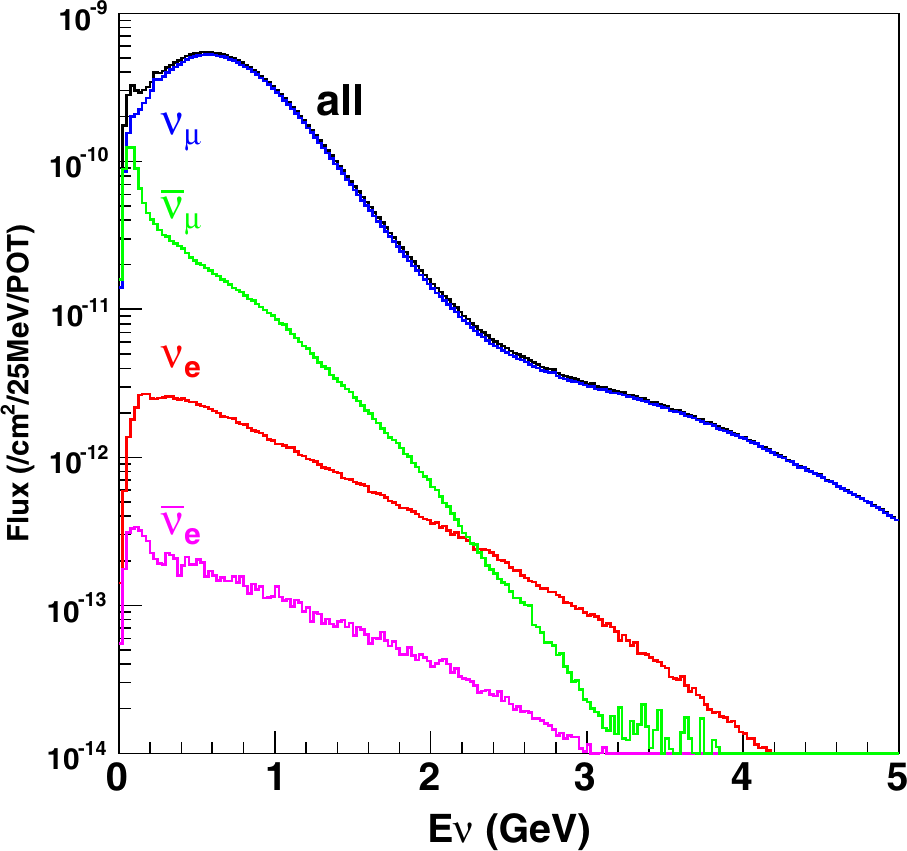
\includegraphics[scale=0.25]{pics/fluxprediction}
  \caption{Neutrino flux predictions from the \textsc{geant4}/FORTRAN simulation.}
  \label{fig:fluxp}
\end{wrapfigure}

A second, FORTRAN-based Monte Carlo code is responsible for generating the neutrino %
kinematics distributions from meson and muon decays, and for obtaining the final neutrino %
fluxes extrapolated to the detector hall with negligible beam Monte Carlo statistical errors. 
Once produced by the simulation, neutrinos are extrapolated along straight lines %
toward the detector and all neutrinos whose traces cross any part of the active volume are %
considered for the flux predictions.
Based on accurate survey data, the distance between the centre of the beryllium %
target and the centre of the SciBar detector is taken to be \np{99.9}~m, %
with the detector located on beam axis within a tolerance of a few centimetres. 

The neutrino flux prediction at the detector location and as a function %
of neutrino energy is shown in Fig.~\ref{fig:fluxp}.
A total neutrino flux per proton on target of \np{2.2e-8}~cm$^{-2}$ is expected at the %
hall location and in neutrino running mode (positive horn polarity), with %
a mean neutrino energy of \np{0.7}~GeV. 
The flux is dominated by muon neutrinos (93\,\% of total), with small contributions from %
muon antineutrinos (6.4\,\%), and electron neutrinos and antineutrinos (0.6\,\% in total). 
For the neutrino flux predictions, no information from BNB %
(SciBooNE or MiniBooNE) neutrino data was used as experimental input.
The \emph{projected number of protons} incident on the target (POT) per year for the BNB %
is about \np{2e20} POT.
The rates expected per year when running in neutrino mode for one ton of water %
(see section~ref) are about sixteen thousands neutrino interactions, %
where eleven thousands of those would be $\nu_\mu$~CC interactions. 
This spectrum peaks ideally in the region of interest at 700 MeV as a result of the simulation %
shown in Fig.~\ref{fig:fluxp}, and has the target rate of neutrino interactions per year.
Another consideration beyond the rates and spectra of in-detector neutrino interactions %
is the probability of seeing multiple events in one beam spill. 
The number of muon neutrino per spill at the SciBooNE location is found to be significantly %
less than one.
In fact from the preliminary simulations, the neutrino interactions occur%
in the tank approximately every 150 spills of \np{4e12}~POTs. 
Additionally our simulations suggest an externally generated muon enters the tank once %
every $\sim$195~spills. 
These rates are ideal as they ensure single neutrino interactions in the detector.

\section{The Hall}

The experiment is set up in the former site of the SciBooNE experiment~refagain?, %
located 8~m below the surface and the 100~m from the BNB target.
Already existing instrumentation in the hall is borrowed by the ANNIE experiment.

\subsection{Water tank}

\begin{wrapfigure}{R}{0.5\textwidth}
  \centering
  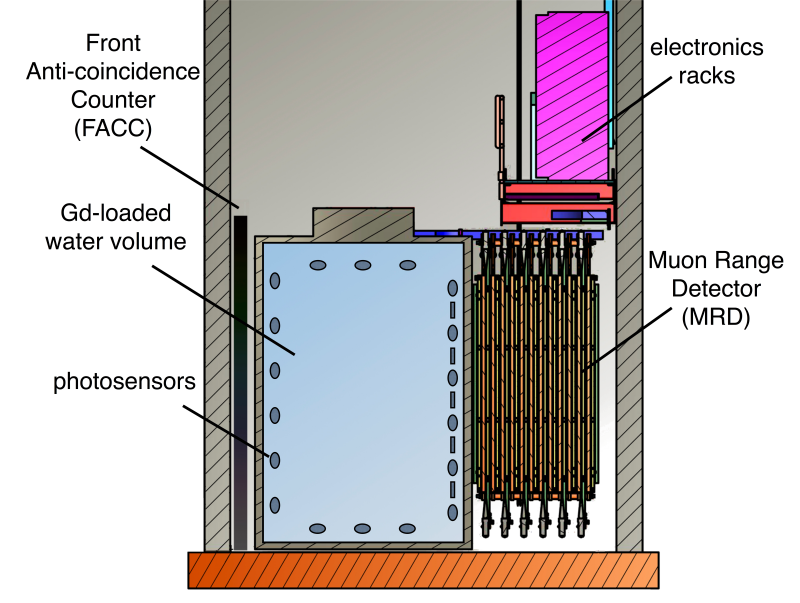
\includegraphics[scale=0.25]{pics/ANNIEreduced2}
  \caption{Schematic of the experimental hall.}
  \label{fig:anniehall}
\end{wrapfigure}

 The main component of the experiment is the water tank, built and installed in the hall.
 It consists of a welded steel water tank, which dimensions are 10~ft (slightly more than three metres) %
 of diameter per 13~ft (nearly four metres) of height, enclosing roughly 23 tonnes of water.
 The characteristic dimension of the tank can be compared to the diagonal of the cylinder, %
 which is about five meters.
 It corresponds to circa seventeen light-nanoseconds.
 The inner volume is lined with a black, water tight plastic bag and outfitted with %
 a PVC inner support structure mounted with 60 PMTs, and capable of ultimately housing several %
 hundred photo-sensors. 
 The tank is filled with pure water and used in conjunction with a smaller %
 acrylic vessel containing Gd-loaded scintillator to measure neutron backgrounds, called %
 Neutron Volume Capture (NCV).
 Due to its two orders of magnitude smaller volume compared to Super-Kamiokande, %
 ANNIE’s water transparency requirements are less stringent: %
 ANNIE needs only to keep a transparency about 25 meters to lose less than 10\,\% of the light, %
 as opposed to SK’s effective water attenuation length of 90 meters.
 The ANNIE water volume requires a source of dry nitrogen in order to suppress the growth of %
 biologics in the water.
 This nitrogen is bubbled through the water during fill and afterwards a blanket of nitrogen %
 will be maintained above the surface of the water. 
 The re-circulation is kept as low as necessary to maintain a pure N$_2$ environment.
 ANNIE also relies on the plastic liner to prevent ions, that might compromise transparency, %
 from leaching into the water from the tank walls.
 Water quality is supposed to be monitored using the detected light intensity from cosmic ray muons.
 
 \begin{wrapfigure}{l}{0.4\textwidth}
   \centering
   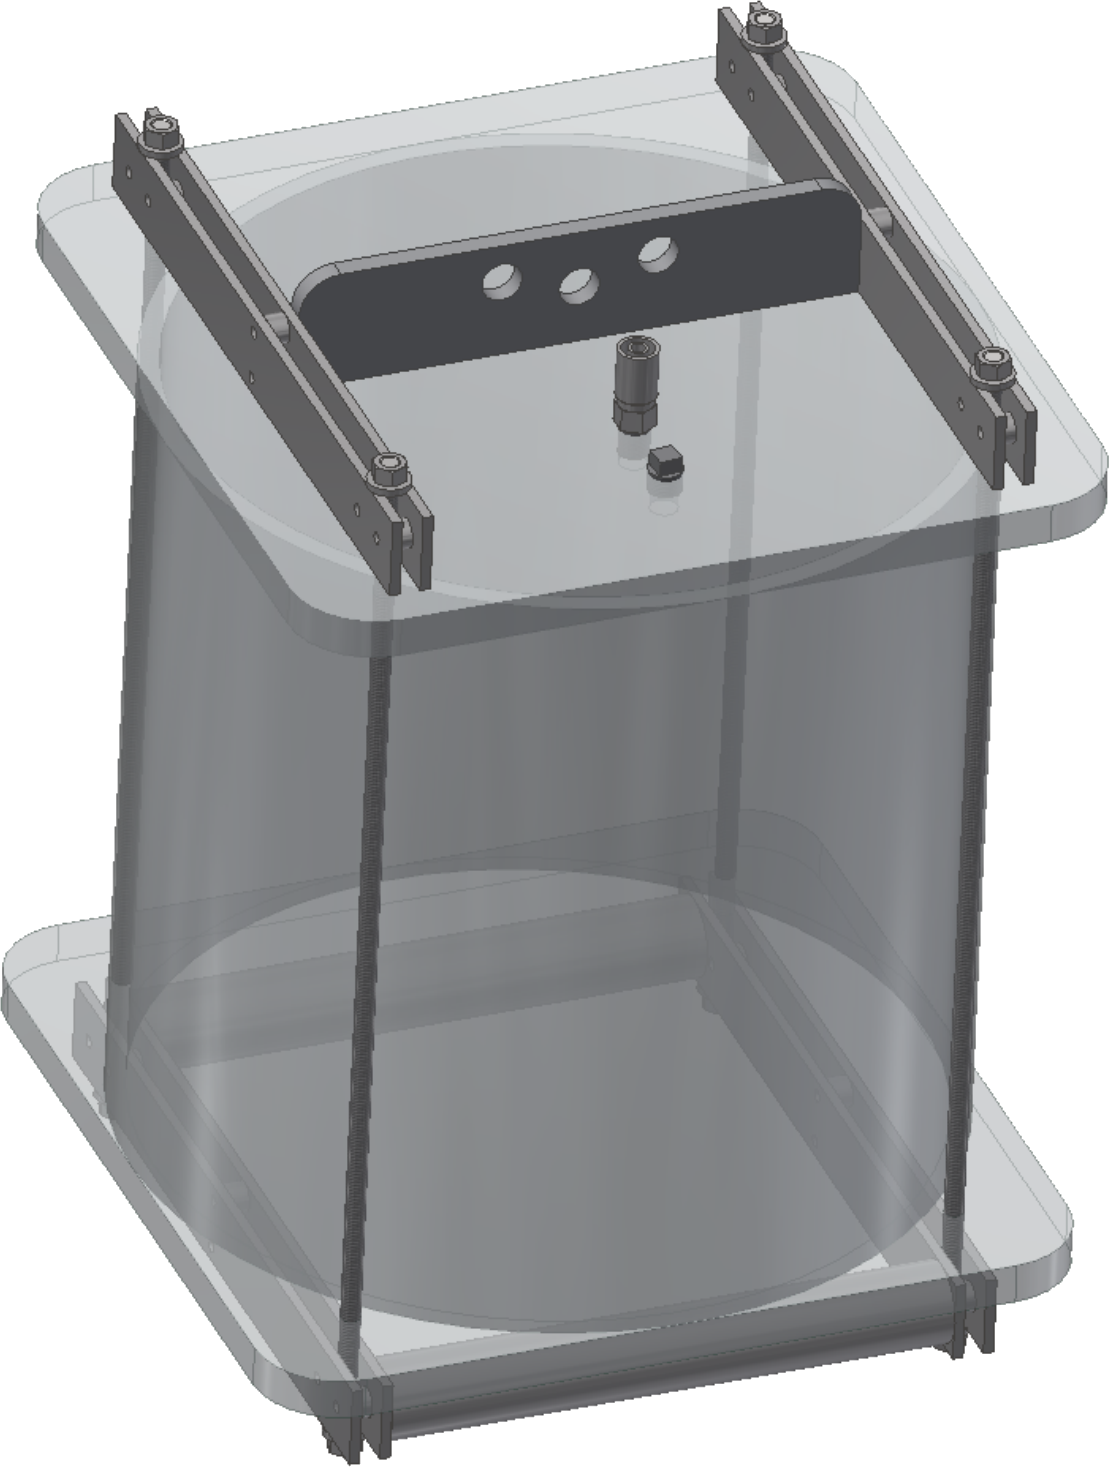
\includegraphics[scale=.15]{pics/ncv}
   \caption{Design of the NCV.}
   \label{fig:ncv}
 \end{wrapfigure}

 A concentrated solution of high-quality (99.99\% TREO\footnote{TREO expresses the %
   Total Rare Earth Oxide percentage in the element.}) gadolinium sulphate %
 $\mathrm{Gd}_2(\mathrm{SO}_4)_3$ will be mixed in a portable polypropylene barrel with pure water.
 The available 50 kg of Gd are enough for one test loading (4~kg) and %
 one full loading (40~kg), with 6~kg left over for various other studies and tests.
 Thanks to the complex of water re-circulation system, the Gd-loaded water can be removed %
 and stored in a secondary tank, then returned and re-purified with minimal loss of Gd, %
 between ANNIE's runs.
 Upon completion of the experiment the gadolinium can be easily recovered using a %
 portable demineraliser.
 Measurement of neutron background will be possible thanks to the NCV.
 It consist of a moveable \np{2.5}~cm thick, 50~cm$\times$50~cm transparent acrylic vessel, %
 which holds 100~L of Gd-doped \textsc{ej-335} liquid scintillator, %
 specialised for neutron detection.
 The light spectrum is shown in Fig.~\ref{fig:ej335}.

 \begin{figure}[]
   \centering
   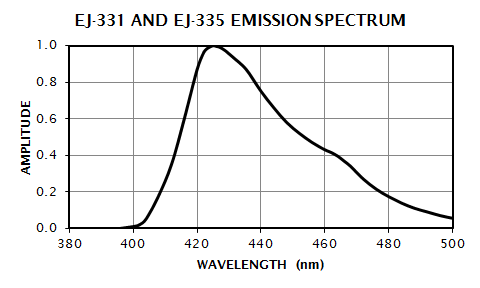
\includegraphics[scale=0.60]{pics/ej335}
   \caption{\textsc{ej-335} emission spectrum. This scintillator contains mineral oil %
 substituted for some of the aromatic solvent for purposes of higher hydrogen content %
 and higher flash point for use in very large tanks. The gadolinium content is 0.25\% by weight.
 The wavelength of peak emission is 424~nm.}
   \label{fig:ej335}
 \end{figure}

 The vessel is weighted so as to have a negative buoyancy.
 Position dependence of the neutron rates from different overburdens of water can be %
 studied by raising and lowering the NCV and translating it along the beam axis.

\subsection{Photodetectors}
\label{2.2.1}
 The core of the experiment is the Cherenkov light detection.
 The coverage provided by 60 8\inch~PMTs borrowed from the WATCHBOY experiment\footnote{The %
   WATCHBOY experiment was designed to measure the rate of radionuclide production in water %
   created by muon spallation. Three primary nuclei of interest, $^{11}$Li, $^8$He, and %
   $^9$ Li, can produce a high energy beta particle in coincidence with a neutron, thus mimicking %
   an antineutrino induced inverse beta decay. The experiment was constructed in 2013 at the %
   Kimbalt on Underground Research Facility (KURF) in Virginia, US.} is enough %
   for the Phase I.
 The photomultipliers are mounted in a frame on the bottom of the tank, facing upward.
 The frame is designed to support both the weight of the phototubes in gravity as well as the %
 buoyant forces in water. 

 As noted earlier, the necessary photo-coverage to reconstruct events in water %
 will be achieved in ANNIE Phase II by:
 \begin{itemize}
   \item reusing the 8\inch~Hamamatsu PMTs recovered from ANNIE Phase I.
   \item purchasing new High Quantum Efficiency (HQE) 10\inch~Hamamatsu PMTs;
   \item employing refurbished 11\inch~Electron Tubes Enterprise PMTs~ref[arXiv:1512.06916v2].
 \end{itemize}
 
 \begin{figure}
   \centering
   \subfloat[8\inch~Hamamatsu R5912.]{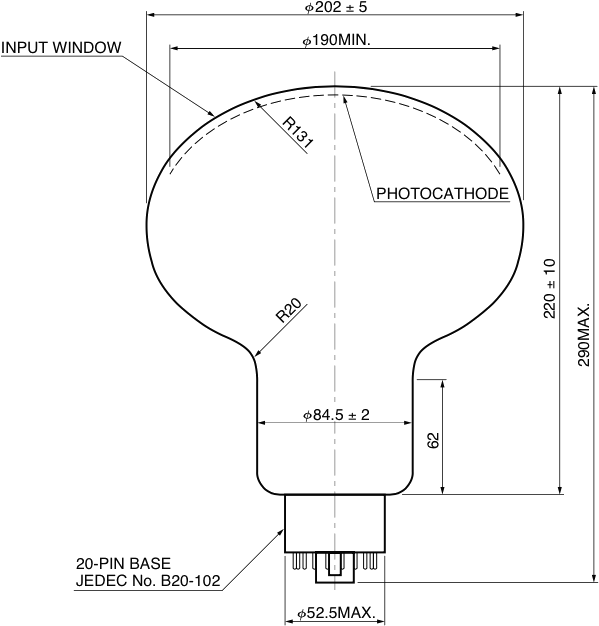
\includegraphics[scale=.2]{pics/8inch}} \qquad
   \subfloat[10\inch~Hamamatsu HQE R7081.]{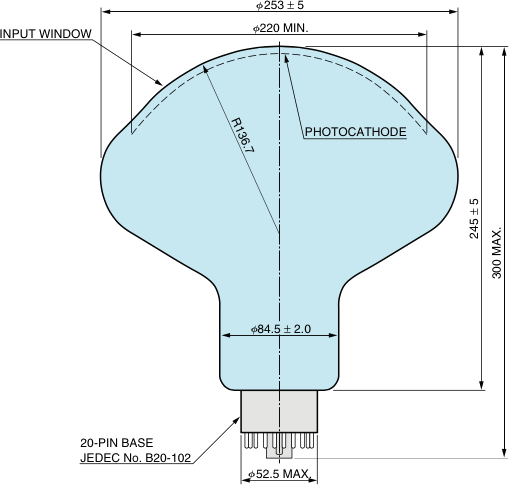
\includegraphics[scale=.2]{pics/10inch}} \qquad
   \subfloat[11\inch~ETEL D748KFLB.]{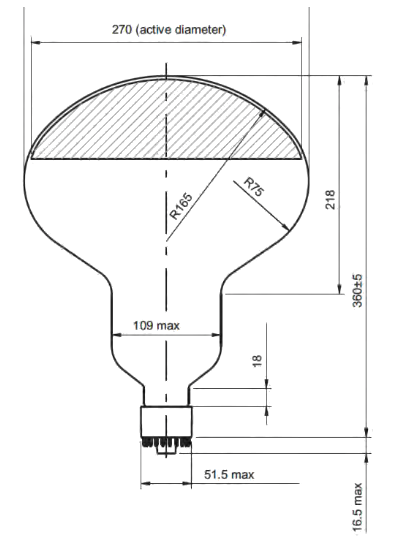
\includegraphics[scale=.2]{pics/11inch}}
   \caption{Schematic of the PMTs employed in the experiment.}
   \label{fig:pmt}
 \end{figure}

 In order to determine the necessary photocathode coverage, a series of simulations has been run %
 with different sizes and numbers of PMTs.
 These full simulations consider neutron captures on both Gd (90\,\%) and the hydrogen from %
 the water (10\,\%).
 After cost and availability are taken into account, it is found that the detection can be %
 optimised by using 58 8\inch~tubes, 20 11\inch~tubes, and 45 HQE 10\inch~tubes.
 Detection probability depends on the number of PMTs hit per neutron capture. 
 Gadolinium captures typically produce several photons, therefore the probability of observing %
 enough hits to detect the event is related to the number of photoelectrons produced.
 This number is strictly correlated with the number of hits.
 The predictions agree well with a simple scaling argument based on measurements %
 at Super-Kamiokande.
 Using the planned mix of 11\inch~tubes, 8\inch~tubes, and HQE 10\inch~tubes, it is found that %
 5 (good correlation) and 10 (strong correlation) photoelectrons are produced respectively %
 99\,\% and 94\,\% of the time.
 
 \textcolor{red}{Have to improve LAPPDs section, but how much?}
 Precise vertex reconstruction will be required for the next stages of the experiment.
 In addition to the PMT coverage improvement, the use of advanced, high resolution photodetectors %
 could have a transformative impact on future neutrino detectors relying on light collection.
 The most promising technology, selected for ANNIE, is the Large Area Picosecond Photodetector %
 (LAPPD), a microchannel plate (MCP) based photomultiplier.
 It can achieve single photoelectron time resolutions less than 100~ps and spatial imaging %
 capabilities to within a single centimetre.
 This provides a much crisper detection of the Cherenkov ring edge and greatly improves the %
 ability to distinguish between closely separate rings.
 On the other hand, conventional PMTs have time resolution of the order of the nanosecond and act %
 as a single pixel, despite the large active area.
 The combination of LAPPDs and PMTs allows the detector to work as a tracking detector, %
 with track and vertex reconstruction approaching size scales of just a few centimetres.
 It also favours the reconstruction of events very close to the wall of the detector, %
 thanks to the small thickness of the LAPPDs (less than \np{1.5}~cm).
 The fiducial volume is thus maximised.
 The LAPPD capabilities also translate into better energy resolution and better discrimination %
 between dark noise and photons from neutron captures.

 {\textcolor{green}{I should put this in ``physics of experiment'' section.}
 \color{blue}
 The maximum transit time for direct light to travel in the ANNIE tank is less than 20 ns.
 The difference in transit time between two photons arriving at the same photosensor from two %
 different forward-pointing tracks is just a few nanoseconds. 
 This is illustrated in Fig 6. 
 For one LAPPD at the centre of overlapping Cherenkov rings, the time separation between photons %
 from a muon and a pion is less than a nanosecond. 
 Time resolutions of 100 and 300 picoseconds are sufficient to resolve that separation. 
 That time separation would be even larger at the photon hits further away from the overlap region. 
 As time resolutions approach the nanosecond scale, typical of conventional PMTs, %
 causal differences between the tracks get significantly washed out.
 Time resolution, however, is not the only essential characteristic. 
 Spatial granularity and short single-PE detector response are also critical.
 Much of the information embedded in overlapping Cherenkov rings can only be extracted %
 if each individual photon is measured independently.
 Conventional large area PMTs are single anode detectors. 
 Moreover the rise times of PMT pulses are comparable to the time differences between %
 the photons being measured. 
 LAPPDs have a fine-grained 30 stripline anode and a single PE response with a rise time %
 of a few hundred picoseconds.
 Large Monte Carlo ensembles show that photon pileup on LAPPDs is low enough that we typically %
 see only one or two hits per channel. 
 Thus, each photon can individually be measured.
 Our preliminary studies show that 20 LAPPDs can provide sufficient coverage and have well-suited %
 performance characteristics for addressing the challenges of WCh reconstruction in a small volume. 
 Better reconstruction could be possible as larger numbers of LAPPDs become available.
 Reaching a 10\,\% isotropic coverage would allow not only from identifying multi-track %
 events but in also identifying the constituent particles and the exact topology potentially %
 expanding the physics reach of the experiment.}

 \subsection[Veto and MRD]{Veto system and Muon Range Detector}
 \label{2.3}
 \textcolor{red}{mostly ok, I guess I have every information.}

 ANNIE is composed of two more detectors other than the water tank in the hall: the Veto system %
 and a muon detector.

 The Veto is provided by a Forward Anti-Coincidence Counter (FACC) consisting of two layers %
 of overlapping scintillating paddles.
 Each layer employes 13 paddles to detect charged particles produced in the dirt %
 upstream of the hall or muons from the BNB, which hasn't decayed.
 This allows the rejection of events in the tank unrelated to neutrino interactions.
 It employes 2\inch~PMTs to read the signals from the scintillator.

 \begin{wrapfigure}{L}{0.5\textwidth}
   \centering
   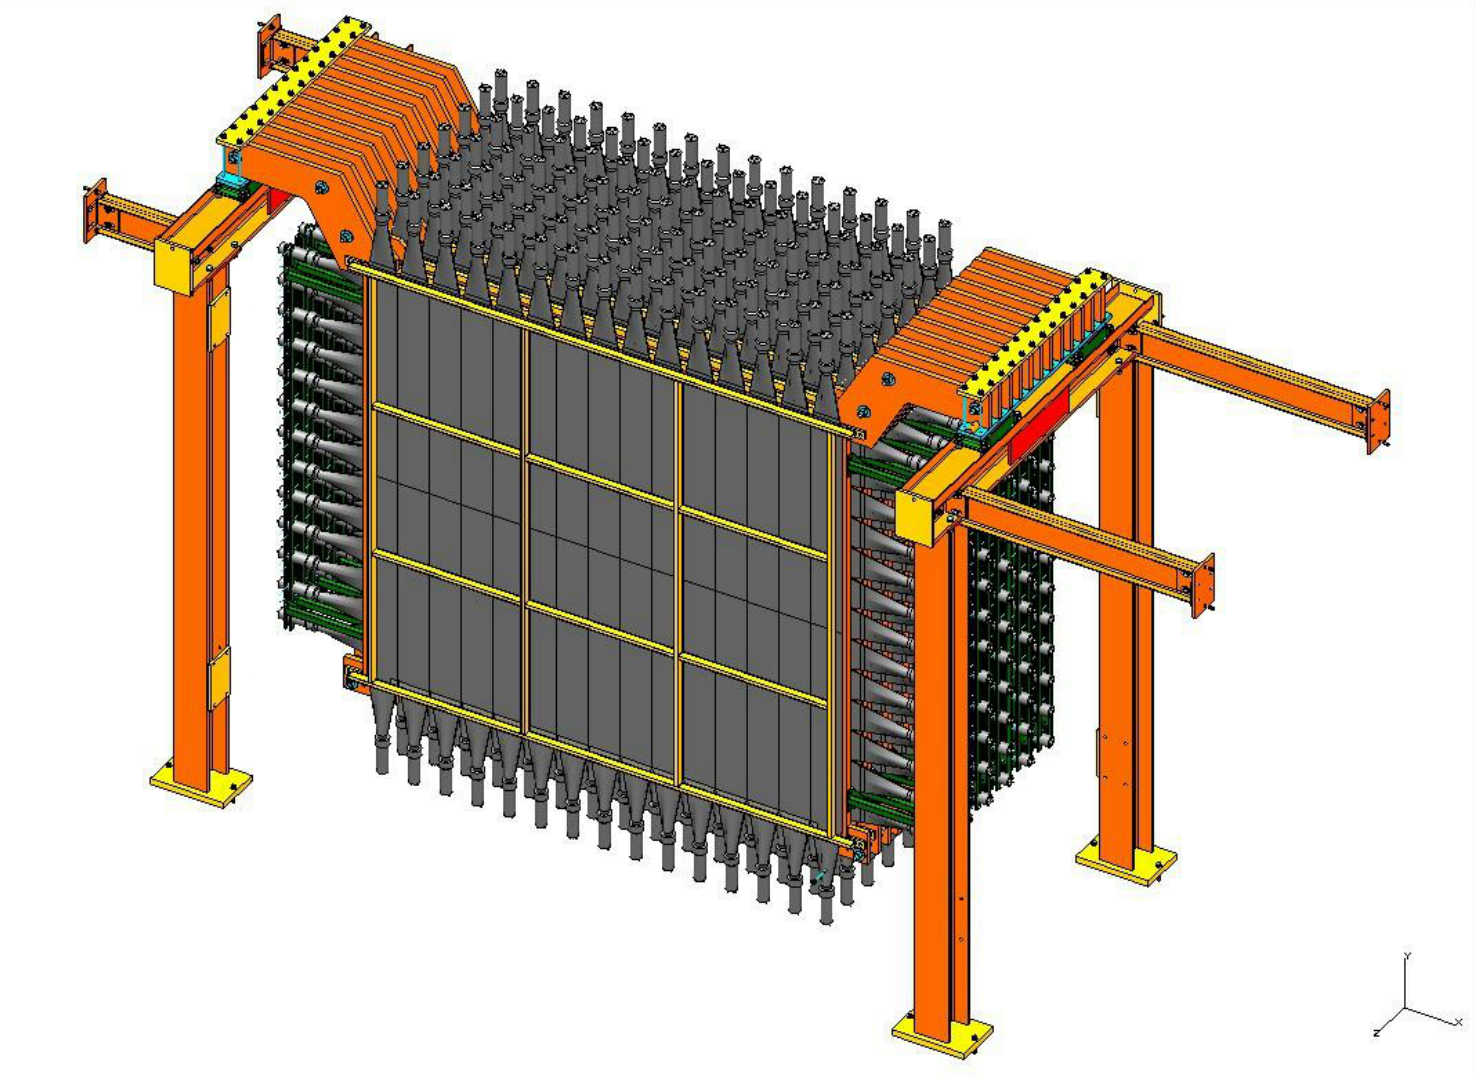
\includegraphics[scale=.15]{pics/pag23Nakajimathesis}
   \caption{Drawing of the MRD.}
   \label{fig:mrd}
 \end{wrapfigure}
 
 An iron-scintillator sandwich, inherited from the SciBooNE experiment, is also in the hall.
 The Muon Range Detector (MRD) is used to range out and fit the direction of daughter muons %
 produced by CCQE interactions in the water target.
 Its schematic drawing is shown in Fig.~\ref{fig:mrd}.
 The muon's energy can be reconstructed thus giving also a handle on the neutrino energy.
 The MRD is designed to measure the momentum of muons up to 1.2 GeV/c using the range measurement.
 It consists of 12 iron plates and 13 alternating horizontal and vertical scintillator planes.
 Each iron plate is 5~cm thick, and covers an area of 274\,$\times$\,305~cm$^2$. 
 The total mass of absorber material is approximately 48~tonnes, while the detector weighs about %
 sixty tonnes.
 The density of a spare iron plate has been measured at several positions of the plate, %
 to be $\np{7.841}\,\pm\,\np{0.002}$~g/cm$^3$. 
 Each scintillator plane consists of 20~cm wide, 6~mm thick scintillator paddles, as %
 illustrated in Fig.~\ref{fig:paddle}.
 Each vertical plane is comprised of 138~cm long paddles, arranged in a 2\,$\times$\,15 %
 array to have an active area of 276\,$\times$\,300~cm$^2$. 
 On the other hand, each horizontal scintillator plane consists of 155~cm long paddles, %
 arranged in a 13\,$\times$\,2 array to have an active area of 260\,$\times$\,310~cm$^2$. 
 In total, 362 paddles, 182 vertical and 180 horizontal, are used in the MRD. 
 The scintillator paddles are read out by five types of 2\inch~PMTs; the vertical
 planes consist of Hamamatsu 2154-05 and RCA 6342A PMTs, the horizontal planes consist of EMI %
 9954KB, EMI 9839b and 9939b PMTs.
 All PMTs used for horizontal modules have 14 stage dynodes, while those used for vertical modules %
 have 10 stage dynodes. 
 This choice is due to space limitations.
 Hence, the PMTs used for the vertical planes have relatively low gain and efficiency compared %
 to that used or horizontal planes. 
 To ensure the same efficiencies, the vertical modules are amplified by the factor of 10 %
 using LeCroy 612 amplifiers.
 
 \begin{figure}[]
   \centering
   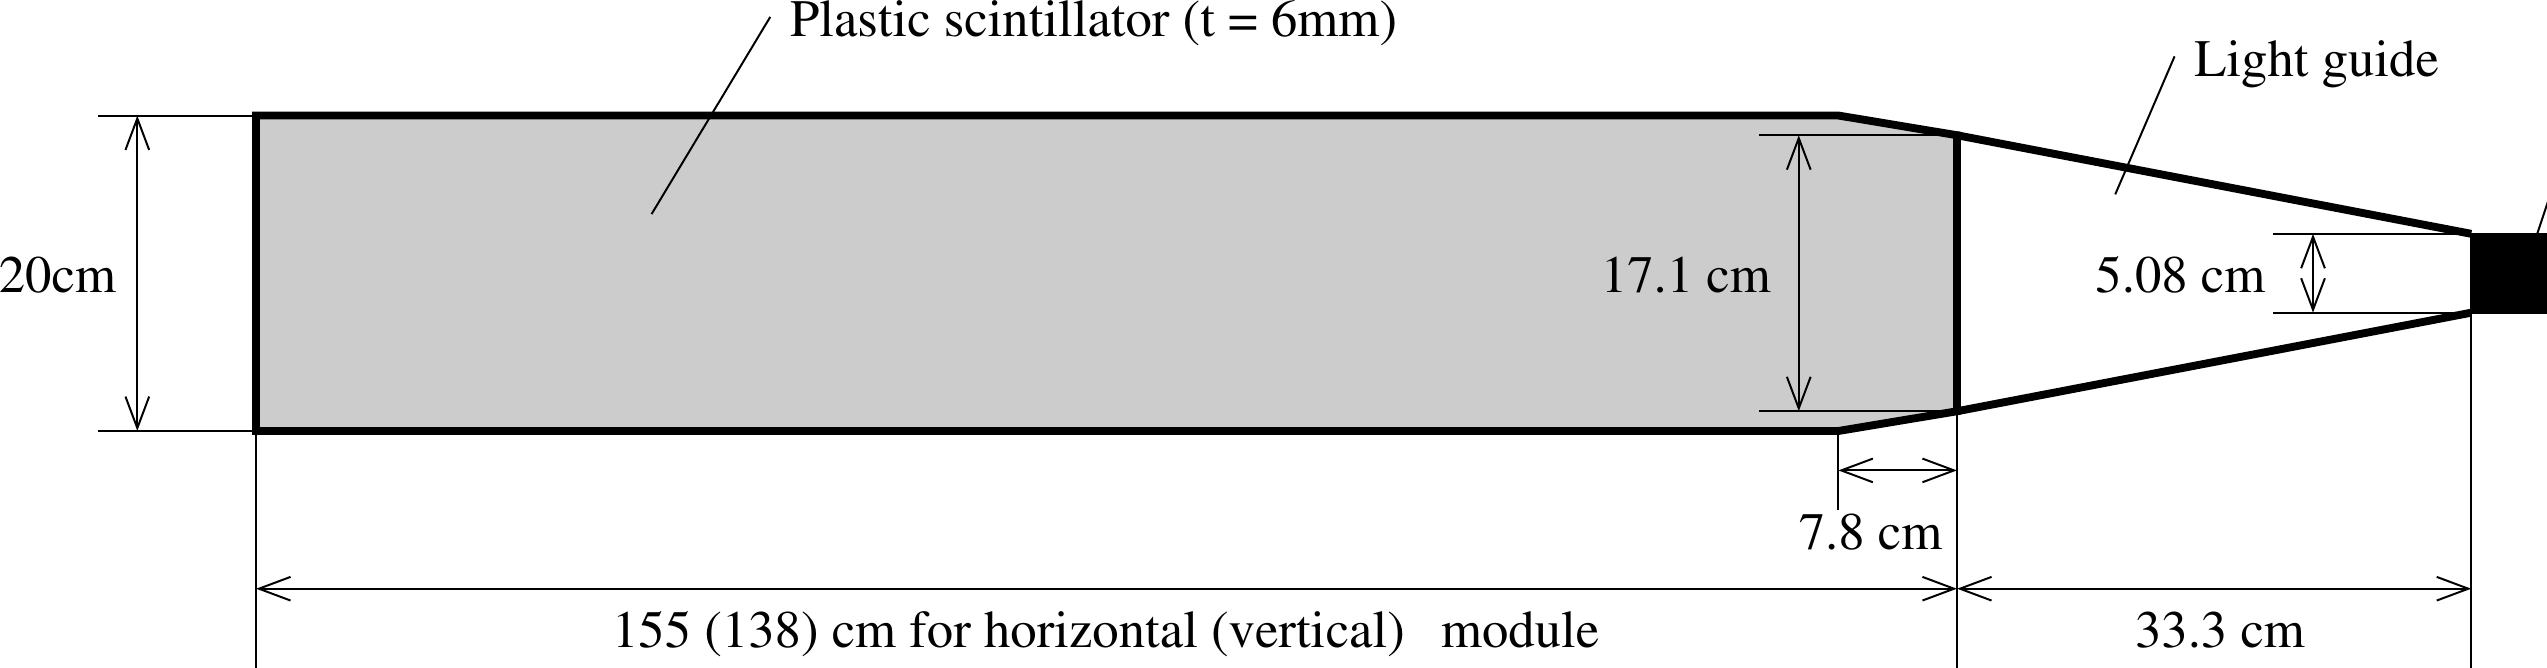
\includegraphics[scale=0.20]{pics/pag24Nakajimathesis}
   \caption{Paddle used for the MRD.}
   \label{fig:paddle}
 \end{figure}

 As far as the electronics are concerned, the FACC and MRD are essentially the same system. 
 Both detectors are composed of scintillating paddles and small phototubes, and both detectors follow
 the same rectilinear geometry.
 The FACC consists of two layers of 13 horizontal paddles. 
 On the MRD side, only a fraction of the detector is operation for Phase I of ANNIE.
 One vertical and one horizontal layer of the MRD (the second and the third layers, respectively) %
 are read.
 \emph{Layer 2} consists of two sets of 13 horizontal paddles, while \emph{Layer 3} consists of two %
 sets of 15 paddles.
 The number of needed readout channels from these two subsystems are
 \begin{itemize}
   \item 26 channels for the forward Veto;
   \item 26 channels for \emph{Layer 2} of the MRD;
   \item 30 channels for \emph{Layer 3} of the MRD;
 \end{itemize}
 for a total of 82 channels.

 In place of the full CAMAC electronics implementation (see section~ref), the two detectors signals %
 are summed and read by VME electronics (section~ref) to give a primary handle on these devices.
 CAMAC electronics (see section~ref) is employed to read these channels.
